\documentclass[12pt,a4paper]{article}
\usepackage[utf8]{inputenc}
\usepackage[german]{babel}
\usepackage[T1]{fontenc}
\usepackage{times}
\usepackage{url}
\usepackage{color}
\usepackage{setspace}
\usepackage{pbox}
\usepackage{graphicx}
\usepackage{adjustbox}
\usepackage{enumerate}
\usepackage{amsmath}
\usepackage{subfigure}
\usepackage{amsfonts}
\usepackage{amssymb}
\usepackage{float}
\usepackage{stix}
\usepackage{xcolor}
\newcommand{\red}[1]{\textcolor{red} {#1}}
\newcommand{\blue}[1]{\textcolor{blue} {#1}}
\newcommand{\green}[1]{\textcolor{green} {#1}}
\newcommand{\yellow}[1]{\textcolor{yellow} {#1}}
\newcommand{\nl}{\\[0.1cm]}
\newcommand{\floor}[1]{\lfloor #1 \rfloor}
\title{Zusammenfassung Software-orientierte Informatik}
\author{Henrik Tscherny}
\begin{document}
\maketitle
\tableofcontents

\section{Systeme}
Ein System ist ein natürliches oder künstliches Gebilde, welches aus Eingangssignalen ($E$) ein Ausgangssignal ($A$) macht. Das System besitzt zudem einen inneren Zustand, der durch Zustandsgrößen ($\vec{Z}$) beschrieben wird. Eine Systemfunktion ($F$) legt fest wie das Eingangssignal in das Ausgangssignal umgewandelt wird ($\vec{A} = F(\vec{E}, \vec{Z},...)$)

\paragraph{Statische Systeme}
Der Output zum Zeitpunkt t ($y(t)$) ist nur von dem zu gleichen Zeitpunkt am Input anliegenden Wert ($x(t)$) abhängig. Innere Zustände ($\vec{Z}$) sind egal. die dazugehörige Funktion $y=f(x)$ nennt man statische Kennlinie.

\paragraph{Dynamische Systeme}
Der Output ($y(t)$) ist von dem am Input anliegenden Signal ($x(t)$) und dem inneren Zustand des Systems ($\vec{Z}$) abhängig. Dabei kann man sich den inneren Zustand als eine Art Gedächtnis vorstellen

\paragraph{Lineare Systeme}
Ein System ist linear, wenn der Überlagerungssatz/Superpositionsprinzip gilt, bzw nicht-linear falls dieser nicht gilt, d.h. Stellt man den Input als die Summe von zwei verschiedenen Inputs dar, so kann man auch den Output als die Summe der beiden Outputs darstellen.\\
$f(x_1 + x_2) = f(x_1) + f(x_2) \Rightarrow y(t) = f(x_1(t) + x_2(t)) = f(x_1(t)) + f(x_2(t))$\\
lineare Systeme werden durch lineare Differenzialgleichungen mit konstanten Koeffizienten beschrieben
\begin{figure}[H]
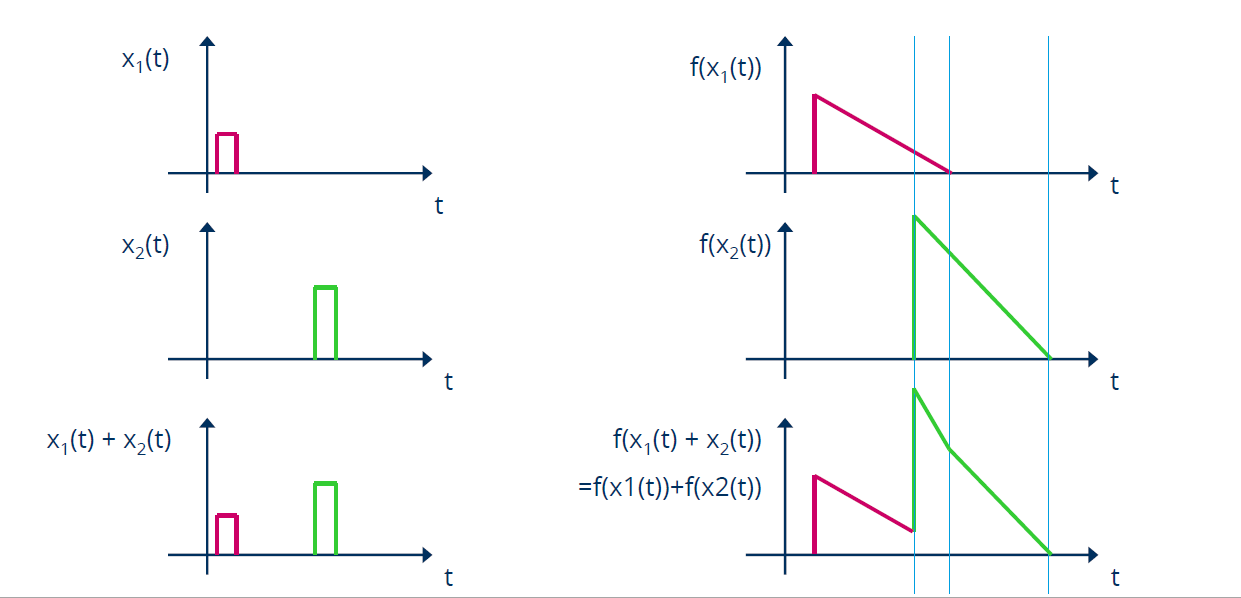
\includegraphics[scale=0.3]{./resources/linear-system.png}
\caption{Veranschaulichung des Superpositionsprinzips}
\end{figure}

\paragraph{Zeit(in)variante Systeme}
Ändern sich die Systemeigenschaften sich nicht mit der Zeit, d.h. es gilt das Verschiebungsprinzip ($y(t-t_0) = f(x(t-t_0))$), ist das System zeitinvariant, andernfalls ist es zeitvariant

\paragraph{Kausales System}
Der Output ist nur von den aktuellen und vergangenen Inputs abhängig, Sprung- und Impulsantwort sind gleich 0 für $t < 0$, gilt dies nicht ist das System akausal.
\begin{itemize}
\item schwach kausal
\begin{itemize}
\item reagiert auf Input x immer mit gleichem Output y
\end{itemize}
\item stark kausal
\begin{itemize}
\item reagiert auf ähnlichen Input x mit ähnlichem Output y
\end{itemize}
\end{itemize}

\subsection{Verknüpfung von Systemen}

\paragraph{Reihenschaltung}
\hspace{1pt}
\begin{figure}[H]
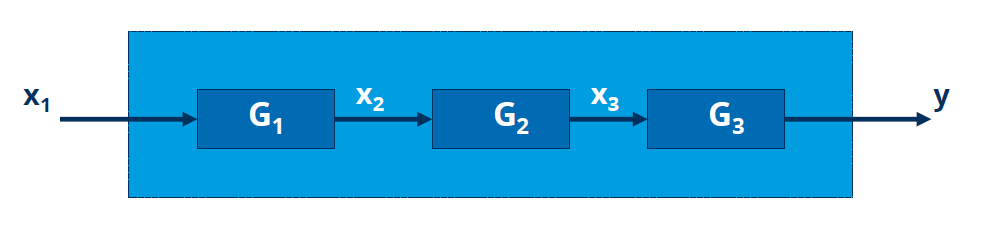
\includegraphics[scale=0.5]{./resources/reihenschaltung.png}
\end{figure}
\begin{tabular}{|c|c|}
\hline
\textbf{statisches System} & \textbf{dynamisches System} \\
$\displaystyle k_{ges} = \prod_{i=1}^n k_i = \frac{\text{output}}{\text{input}}$ & $\displaystyle G_{ges}(f) = \prod_{i=1}^n G_i(f) = \frac{\text{input}(f)}{\text{output}(f)}$ \\
\hline
$G_i = k_i$: statische Übertragungsfaktor & $G_i(f)$: Übertragungsfunktion des Teilsystems i \\
\hline
\end{tabular}
\newpage
\paragraph{Parallelschaltung}
\hspace{1pt}
\begin{figure}[H]
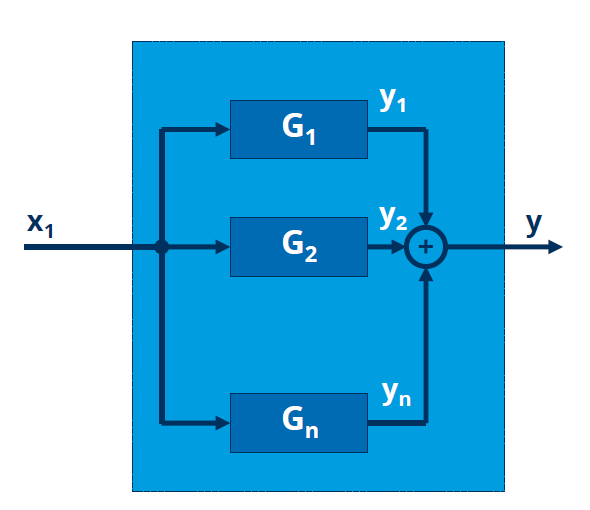
\includegraphics[scale=0.5]{./resources/parallelschaltung.png}
\end{figure}
\begin{tabular}{|c|c|}
\hline
\textbf{statisches System} & \textbf{dynamisches System} \\
$\displaystyle k_{ges} = \sum_{i=1}^n k_i$ & $\displaystyle G_{ges}(f) = \sum_{i=1}^n G_i(f)$\\
\hline
$G_i = k_i$: statische Übertragungsfaktor & $G_i(f)$: Übertragungsfunktion des Teilsystems i \\
\hline
\end{tabular}

\paragraph{Rückkopplungsschaltung}
\hspace{1pt}
\begin{figure}[H]
\includegraphics[scale=0.5]{./resources/rückkopplungsschaltung.png}
\end{figure}
\begin{tabular}{|c|c|}
\hline
\textbf{statisches System} & \textbf{dynamisches System} \\
$\displaystyle k_{ges} = \frac{y}{x} = \frac{k_1}{1 \pm k_1 k_2}$ & $\displaystyle G_{ges}(f) = \frac{G_1(f)}{1 \pm G_1(f)G_2(f)}$\\
\hline
\end{tabular}

\subsection{Grundsysteme}
\begin{tabular}{|c|c|c|}
\hline
Type & Differenzialgleichung & Differenzengleichung\\
\hline
\begin{tabular}{c}
Proportionalsystem (P)\\
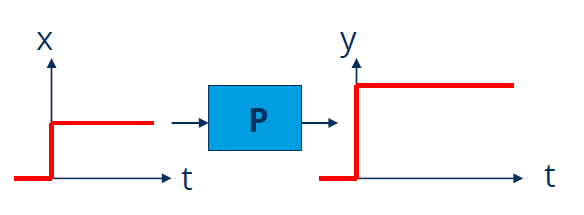
\includegraphics[scale=0.3]{./resources/p-sys.png} 
\end{tabular} & $\frac{dy}{dx} = K_p$ & $y(i) = K_p x(i)$\\
\hline
\begin{tabular}{c}
Integralsystem (I)\\
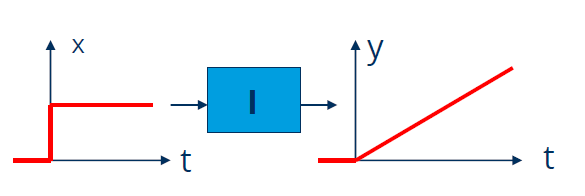
\includegraphics[scale=0.3]{./resources/i-sys.png}
\end{tabular} & \begin{tabular}{c}
$\frac{dy}{dt} = K_I x(t)$\\
$\displaystyle y(t) = K_I \int_0^t x(\tau) d\tau$
\end{tabular} & $y(i) = TK_I x(i) + y(i-1)$ \\
\hline
\begin{tabular}{c}
Differentialsystem (D) \\
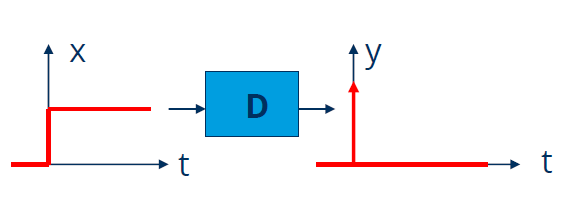
\includegraphics[scale=0.3]{./resources/d-sys.png}
\end{tabular} & $\frac{dx}{dt}K_D = y(t)$ & $y(i) = \frac{K_D}{T}(x(i)-x(i-1))$\\
\hline
\begin{tabular}{c}
Totzeitsystem ($T_t$)\\
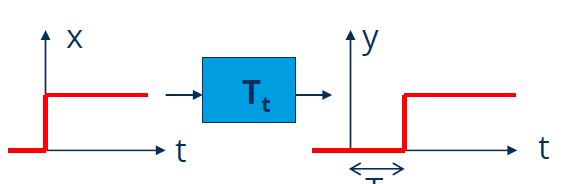
\includegraphics[scale=0.3]{./resources/tt-sys.png}
\end{tabular} & $y(t) = x(t-T_t)$ & \begin{tabular}{c}
$y(i) = x(i-n)$\\
$n=\frac{T_t}{T}$
\end{tabular}\\
\hline
\begin{tabular}{c}
Verzögerunssystem ($T_1$)\\
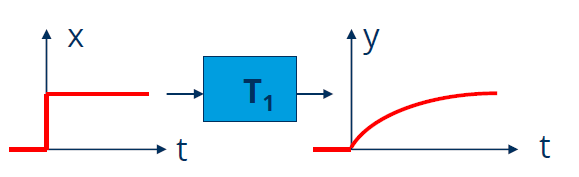
\includegraphics[scale=0.3]{./resources/t1-sys.png}
\end{tabular} & $\frac{dy}{dt}T_1 + y(t) = x(t)$ & \begin{tabular}{c}
$y(i) = (1-\alpha)x(i) +\alpha y(i-1)$\\
$\alpha=\frac{T_1}{T+T_1}$
\end{tabular}\\
\hline
\end{tabular}

\section{Faltung/Konvolution}
Die Faltung beschriebt einen mathematischen Operator ($\ast$) welcher für zwei Funktionen f und g eine dritte Funktion $f \ast g$ liefert.\nl
$\displaystyle (f\ast g)(x) = \int_{\mathbb{R^n}} f(\tau) g(x-\tau)d\tau$\nl
Intuitiv kann man sich die Faltung von zwei Funktionen f und g so vorstellen, dass man die Funktion g entlang der x-Achse schiebt (daher $x-\tau$) und dabei diese über die Funktion f hinweg schiebt. Dabei berechnet man dann in Jedem Schritt die Fläche in welcher sich die beiden Funktionen überlappen. Der Flächeninhalt der Überlappung ist dann der Funktionswert der Funktionswert der Funktion $(f \ast g) (x)$
\flushleft

\textbf{Eigenschaften der Faltung}:
\begin{itemize}
\item Kommutativität: $f \ast g = g \ast f$
\item Assoziativität: $f \ast (g \ast h) = (f \ast g) \ast h$
\item Distributivität: $f \ast (g+h) = (f \ast g) + (f \ast h)$
\end{itemize}
\flushleft
Für den zeitdiskreten Fall gibt es äquivalent zum Faltungsintegral die Faltungssumme:\nl
$\displaystyle f(kT) \ast g(kT) = \begin{cases} 0 & k<0 \\
\displaystyle \sum_{j=0}^k f((k-j)T)g(jT) & k \geq 0
\end{cases}$

\paragraph{Stabilität}
Ein System ist \textbf{BIBO-stabil}, wenn es für jeden beschränkten Input Wert auch nur maximal einen beschränkten 
Output wert liefert\nl
\begin{itemize}
\item zeitkontinuierlich: $\displaystyle \int_{-\infty}^{+\infty} |g(t)|dt < \infty$
\item zeitdiskret: $\displaystyle \sum_{-\infty}^{+\infty} |g(kT)|T < \infty$
\end{itemize}

\subsection{Beispiel}
Faltung der Rechteckfunktion mit sich selbst:\nl

\begin{minipage}{\linewidth}
\centering
\begin{minipage}{0.45\linewidth}
\begin{figure}[H]
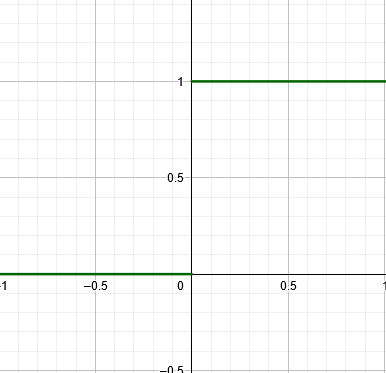
\includegraphics[width=0.9\linewidth]{./resources/einheitssprung_funktion.png}
\end{figure}
\end{minipage}
\hspace{0.05\linewidth}
\begin{minipage}{0.45\linewidth}
\begin{figure}[H]
Sei $u(x) = \displaystyle \begin{cases} 0, & x<\tau \\ 1, & x\geq \tau \end{cases}$\\
der Einheitssprung beginnend ab\\ $x = \tau$
\end{figure}
\end{minipage}
\end{minipage}
\nl

\begin{minipage}{\linewidth}
\centering
\begin{minipage}{0.45\linewidth}
\begin{figure}[H]
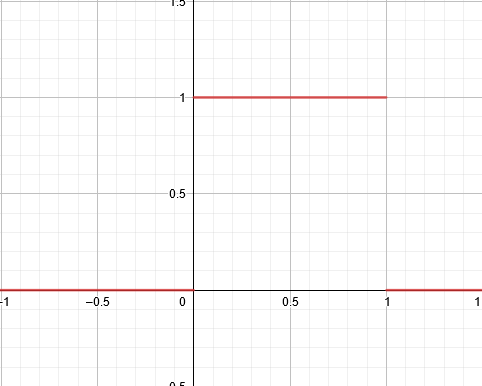
\includegraphics[width=0.9\linewidth]{./resources/rechteck_funktion.png}
\end{figure}
\end{minipage}
\hspace{0.05\linewidth}
\begin{minipage}{0.45\linewidth}
\begin{figure}[H]
Stelle die Rechteckfunktion als die Differenz von zwei Einheitssprüngen dar\\
$r(x) = u(x) - u(x-1)$
\end{figure}
\end{minipage}
\end{minipage}
\nl


\begin{minipage}{\linewidth}
\centering
\begin{minipage}{0.45\linewidth}
\begin{figure}[H]
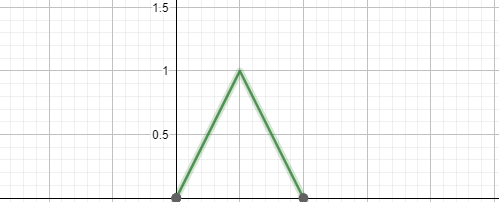
\includegraphics[width=\linewidth]{./resources/rechteck_faltung.png}
\end{figure}
\end{minipage}
\hspace{0.05\linewidth}
\begin{minipage}{0.45\linewidth}
\begin{figure}[H]
Faltung mit sich selbst: $(r\ast r)(x) = \displaystyle \int_{\mathbb{R}^n} r(\tau)r(x-\tau)d\tau = \begin{cases} 0,& x<0 \\ 2x, & 0 \leq x \leq 0.5 \\ -2(x-1), & 0.5 \leq x \leq 1 \end{cases}$
\end{figure}
\end{minipage}
\end{minipage}
\nl
Man kann leicht sehen, dass der Wert von $(f \ast f) (0.5) = 1$, da sich dort die beiden Rechteckfunktionen exakt überlagern, somit ist die Fläche gleich 1



\end{document}